\documentclass[a4paper,12pt]{article}
\usepackage[utf8]{inputenc}
\usepackage[T1]{fontenc}
\usepackage{lmodern}
\usepackage[brazilian]{babel}
\usepackage{graphicx}
\usepackage{geometry}
\usepackage{caption}
\usepackage{enumitem}
\usepackage{pdflscape}

\geometry{margin=1in}
\setlist[itemize]{noitemsep,topsep=4pt,leftmargin=*}
\emergencystretch=3em
\title{Modelo Entidade-Relacionamento\\da Aplicação UnB RU}
\author{}
\date{}
\begin{document}
\maketitle
\section*{Introdução}
\begingroup\raggedright
Como parte da Sprint 1, esse documento apresenta a modelagem Entidade-Relacionamento criado baseando-se 
na histórias de usuário. 
\par\endgroup

\section*{Entidades Principais}
\subsection*{1. Usuário}
\begin{itemize}
    \item \textbf{matricula}: Matrícula única de nove dígitos (PK).
    \item \textbf{nome}: Nome do usuário.
    \item \textbf{senha\_hash}: Hash da senha do usuário.
    \item \textbf{perfil}: Estudante, funcionário ou administrador.
    \item \textbf{turno}: O turno, caso funcionario, de trabalho.
    \item \textbf{restaurante}: O restaurante, caso funcionario, de trabalho.
    \item \textbf{saldo}: Crédito disponível.
\end{itemize}
\noindent\textbf{Relacionamento:} Um usuário com perfil de estudante pode realizar 
nenhuma ou várias recargas, tentativas de acesso e inscrições em sorteios do FastPass. 

\subsection*{2. Restaurante}
\begin{itemize}
    \item \textbf{id}: Identificador do restaurante (PK).
    \item \textbf{nome}: Nome do restaurante.
\end{itemize}

\noindent\textbf{Relacionamento:} Um restaurante pode possuir uma ou várias 
catracas e nenhum ou vários cardápios. Cada catraca pertence a um único 
restaurante; um cardápio pode ser compartilhado por vários restaurantes.

\subsection*{3. Catraca}
\begin{itemize}
    \item \textbf{id}: Identificador da catraca (PK).
    \item \textbf{restaurante\_id}: Restaurante associado (FK).
    \item \textbf{piso}: Piso em que a catraca está localizada.
    \item \textbf{modo\_acesso}: normal ou exclusivo fastpass.
\end{itemize}
\noindent\textbf{Relacionamento:} Cada catraca pertence a um restaurante e pode 
registrar nenhuma ou várias tentativas de acesso. 

\subsection*{4. Turno}
\begin{itemize}
    \item \textbf{id}: Identificador único do turno (PK).
    \item \textbf{nome}: Tipo de refeição, como almoço ou jantar.
    \item \textbf{inicio}: Horário de início do atendimento.
    \item \textbf{fim}: Horário de encerramento do atendimento.
    \item \textbf{preco}: Valor da refeição nesse turno.
\end{itemize}
\noindent\textbf{Relacionamento:} Um turno pode possuir nenhum ou vários time-frames, cardápios e acessos. Cada um desses registros se refere a um único turno. Para simplificar a simulação, o preço de cada turno é compartilhado pelos restaurantes.
\subsection*{5. Time-frame}
\begin{itemize}
    \item \textbf{id}: Identificador único do intervalo (PK).
    \item \textbf{turno\_id}: Turno associado (FK).
    \item \textbf{inicio}: Horário inicial do intervalo.
    \item \textbf{fim}: Horário final do intervalo.
\end{itemize}
\noindent\textbf{Relacionamento:} Cada time-frame pertence a um turno e pode 
ser escolhido em nenhuma ou várias inscrições. 
\subsection*{6. Cardápio}
\begin{itemize}
    \item \textbf{id}: Identificador do cardápio (PK).
    \item \textbf{turno\_id}: Turno associado (FK).
    \item \textbf{data}: Data do cardápio.
    \item \textbf{opcao\_padrao}: Descrição dos pratos da opção padrão.
    \item \textbf{opcao\_ovolactovegetariana}: Descrição dos pratos da opção ovolactovegetariana.
    \item \textbf{opcao\_vegetariana\_estrita}: Descrição dos pratos da opção vegetariana estrita.
\end{itemize}
\noindent\textbf{Relacionamento:} Cada cardápio está associado a um ou mais restaurantes, 
uma data e um turno. A associação com restaurantes é muitos-para-muitos e está
representada diretamente no diagrama ER. Na implementação relacional, ela será
armazenada em uma tabela de associação entre restaurante e cardápio.

\subsection*{7. Recarga}
\begin{itemize}
    \item \textbf{id}: Identificador da recarga (PK).
    \item \textbf{usuario\_matricula}: Matrícula do estudante associado a recarga (FK).
    \item \textbf{data\_hora}: Data e horário da recarga.
    \item \textbf{valor}: Valor da recarga.
    \item \textbf{metodo}: Forma do pagamento.
    \item \textbf{status}: pendente, confirmada ou falhou.
\end{itemize}
\noindent\textbf{Relacionamento:} Cada recarga pertence a um estudante, 
que pode possuir várias recargas. 

\clearpage
\subsection*{8. Acesso}
\begin{itemize}
    \item \textbf{id}: Identificador da entrada (PK).
    \item \textbf{usuario\_matricula}: Matrícula do estudante (FK).
    \item \textbf{catraca\_id}: Catraca utilizada (FK).
    \item \textbf{turno\_id}: Turno da refeição (FK).
    \item \textbf{inscricao\_fastpass\_id}: Inscrição no FastPass (FK) (Opcional).
    \item \textbf{data\_hora}: Data e horário.
    \item \textbf{status}: liberado ou bloqueado.
    \item \textbf{passagem\_em}: Data e horário da passagem confirmada.
    \item \textbf{valor\_debitado}: Valor cobrado.
\end{itemize}
\noindent\textbf{Relacionamento:} Cada acesso pertence a um estudante, 
uma catraca e um turno, podendo estar relacionado a uma inscrição FastPass. 
\subsection*{9. Sorteio}
\begin{itemize}
    \item \textbf{id}: Identificador do sorteio (PK).
    \item \textbf{data}: Data referente ao sorteio.
    \item \textbf{status}: aberto, encerrado ou apurado.
\end{itemize}
\noindent\textbf{Relacionamento:} Um sorteio pode receber nenhuma ou várias 
inscrições, inclusive para turnos diferentes. 

\subsection*{10. Inscrição FastPass}
\begin{itemize}
    \item \textbf{id}: Identificador da inscrição (PK).
    \item \textbf{usuario\_matricula}: Matrícula do estudante (FK).
    \item \textbf{sorteio\_id}: Sorteio associado (FK).
    \item \textbf{time\_frame\_id}: Time-frame escolhido (FK).
    \item \textbf{resultado}: pendente, contemplada ou nao contemplada.
    \item \textbf{status\_notificacao}: pendente, falhou ou entregue.
    \item \textbf{notificada\_em}: Data e horário de entrega da notificação.
\end{itemize}
\noindent\textbf{Relacionamento:} Cada inscrição associa um estudante a um sorteio e um time-frame. 
\newgeometry{margin=1.3cm}
\begin{landscape}
\section*{Modelo Entidade-Relacionamento}
O diagrama foi gerado a partir de modelo-er.mmd.
\begin{center}
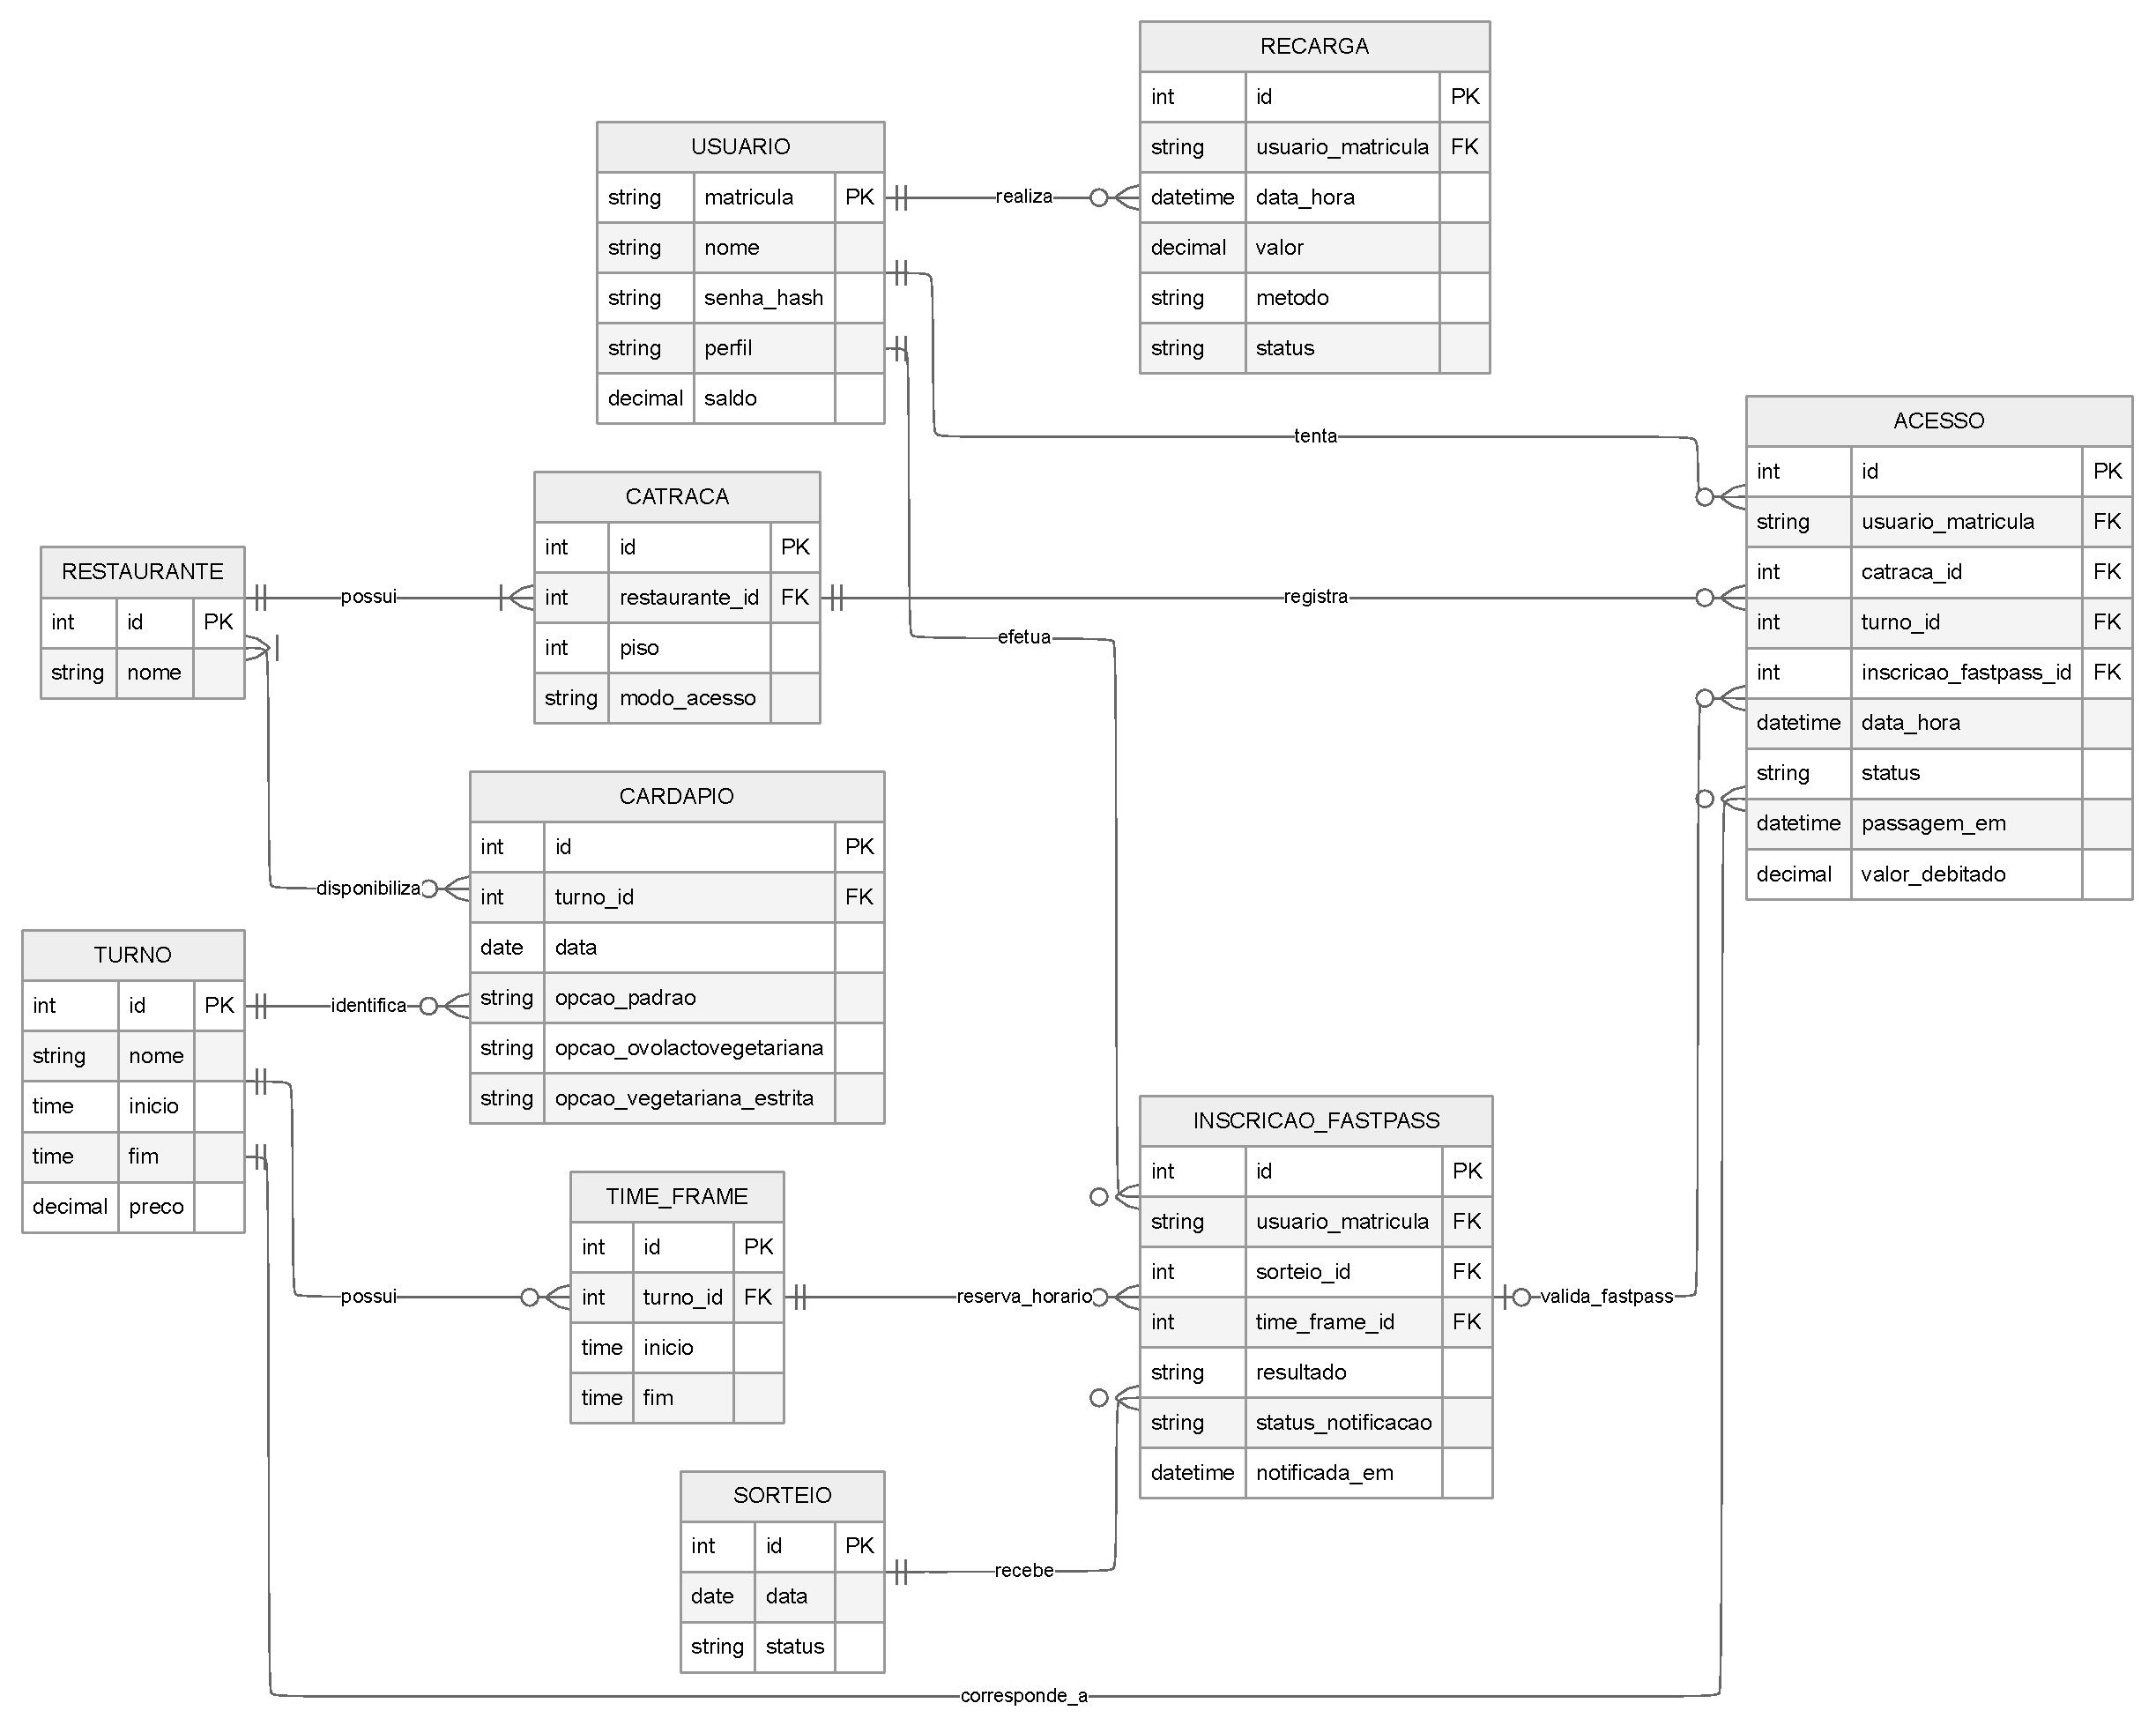
\includegraphics[width=0.98\linewidth,height=14.5cm,keepaspectratio]{modelo-er.pdf}
\captionof{figure}{Modelo entidade-relacionamento da aplicação UnB RU.}
\label{fig:er-unb-ru}
\end{center}
\end{landscape}
\restoregeometry
\section*{Considerações Finais}

O modelo apresentado estrutura uma forma de se representar o banco de dados 
para o RU da UnB com base as histórias especificadas. A imagem utilizada no 
relatório foi feita usando o Mermaid CLI, mas pode ser consultado em modelo-er.mmd.

\paragraph{Uso de IA.} Foi utilizado o Codex com o modelo GPT-6.1 Sol 
no auxilio da especificação do modelo ER em Mermaid e na 
validação da coerência entre a modelagem e as histórias analisadas.
\end{document}
